\section{Geometry}



\subsection*{Vector3d}

\begin{frame}[fragile]
  \frametitle{Specimen Directions - The \MTEX Class \texttt{\bf vector3d}}

  Definition:

\begin{lstlisting}
v = vector3d(1,1,1);    % by Cartesian coordinate
v = sph2vec(theta,rho); % by polar coordinates
v = xvector;            % predefined vectors
\end{lstlisting}

  \medskip

  \begin{columns}
    \begin{column}{8.5cm}

      Calculations:

\begin{lstlisting}
v = [xvector,yvector]; w = v(1);
v = 2*xvector-yvector;
\end{lstlisting}

    \medskip

    Basic Functions:

\begin{lstlisting}
cross(v1,v2), dot(v1,v2)
norm(v), sum(v)
vec2sph(v)
\end{lstlisting}
  \end{column}
  \begin{column}{3cm}
   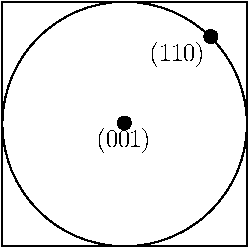
\includegraphics[width=3cm]{pic/vector3d}
  \end{column}
\end{columns}



\end{frame}

\subsection*{quaternion}


\begin{frame}[fragile]
  \frametitle{Rotations - The \MTEX Class \texttt{\bf quaternion}}

Definition:

\begin{lstlisting}
q = quaternion(a,b,c,d);
q = axis2quat(axis,omega);
q = euler2quat(alpha,beta,gamma);
q = euler2quat(phi1,Phi,phi2,'Bunge');
q = Miller2quat([h k l],[u v w],CS);
\end{lstlisting}
%q = idquaternion;

\medskip

\begin{columns}
  \begin{column}{8.5cm}

    Calculations:

\begin{lstlisting}
q = [q1,q2]; q1 = q(1)
q = q1 * q2; w = q * v
\end{lstlisting}

    \medskip

    Basic Functions:

\begin{lstlisting}
omega = rotangle(q)
v = rotaxis(q)
[alpha,beta,gamma]  = quat2euler(q)
\end{lstlisting}

  \end{column}

  \begin{column}{3cm}
    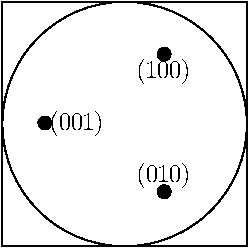
\includegraphics[width=3cm]{pic/quaternion}
  \end{column}

\end{columns}
\end{frame}

\subsection*{Symmetry}
\begin{frame}[fragile]
  \frametitle{Crystal Symmetries - The \MTEX Class \texttt{\bf symmetry}}

  Definition:

\begin{lstlisting}
S = symmetry('triclinic',[a,b,c],[alpha,beta,gamma])
S = symmetry('-3m',[a,b,c],/+'a||x'+/);
S = symmetry('O');
\end{lstlisting}

\medskip

\begin{columns}
  \begin{column}{8.5cm}

Load Symmetry from CIF file:

\begin{lstlisting}
cif2symmetry('quartz.cif')
\end{lstlisting}

\medskip

    Basic Functions:

\begin{lstlisting}
symmetriceVec(SS,v)
dist(CS,SS,q1,q2)
quaternion(CS)
getFundamentalRegion(CS)
\end{lstlisting}
  \end{column}

  \begin{column}{3cm}
    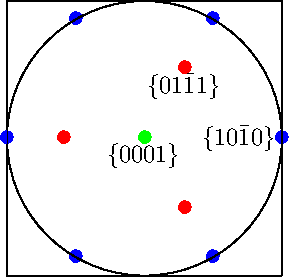
\includegraphics[width=3cm]{pic/sym}
  \end{column}

\end{columns}

\end{frame}

\subsection*{Miller}

\begin{frame}[fragile]
  \frametitle{Crystal Directions - The \MTEX Class \texttt{\bf Miller}}

  Definition:

\begin{lstlisting}
h = Miller(1,0,0,CS);
h = [Miller(1,1,-2,3,CS),Miller(0,1,-1,0,CS)]
h = vec2Miller(v,CS);
\end{lstlisting}

\medskip

\begin{columns}
  \begin{column}{8.5cm}

    Calculations:

\begin{lstlisting}
q * Miller(1,0,0,CS)
q * symeq(Miller(1,0,0,CS))
\end{lstlisting}

    \medskip

    Basic Functions:


    \begin{onlyenv}<1>
\begin{lstlisting}
symeq(h1,h2)
symvec(h)
angle(h1,h2)
plot([h1,h2],'all')
\end{lstlisting}
    \end{onlyenv}

    \begin{onlyenv}<2>
      \lstset{stringstyle=\color{red},emph={antipodal},emphstyle=\em\color{red}}
\begin{lstlisting}
symeq(h1,h2,`antipodal`)
symvec(h,`antipodal`)
angle(h1,h2,`antipodal`)
plot([h1,h2],'all',`antipodal`)
\end{lstlisting}
    \end{onlyenv}

  \end{column}

  \begin{column}{3cm}
    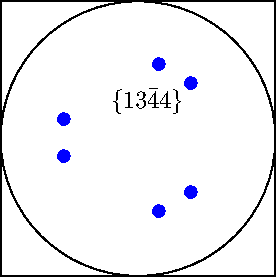
\includegraphics[width=3cm]{pic/miller}
  \end{column}

\end{columns}

\end{frame}

\subsection*{S2Grid}


\begin{frame}[fragile]
  \frametitle{Sets of Specimen Directions - The \MTEX Class \texttt{\bf S2Grid}}

Definition:

\begin{lstlisting}
S2G = S2Grid('regular','resolution',5*degree);
S2G = S2Grid('regular','maxrho',80*degree);
S2G = S2Grid('equispaced','points',10000);
\end{lstlisting}

\medskip

Basic Functions:

\begin{lstlisting}
add, delete, rotate, union, subGrid, refine,
GridLength, getResolution, getRho, getTheta,
polar, vector3d
\end{lstlisting}

\onslide<1->
\begin{center}
  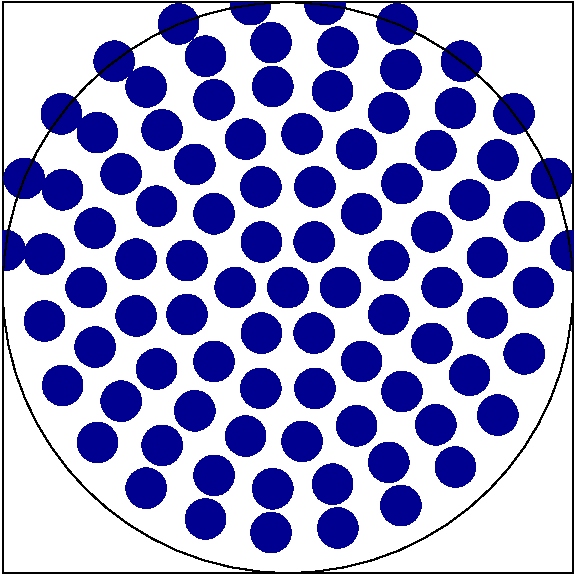
\includegraphics[width=2.5cm]{pic/S2Grid1} \quad
  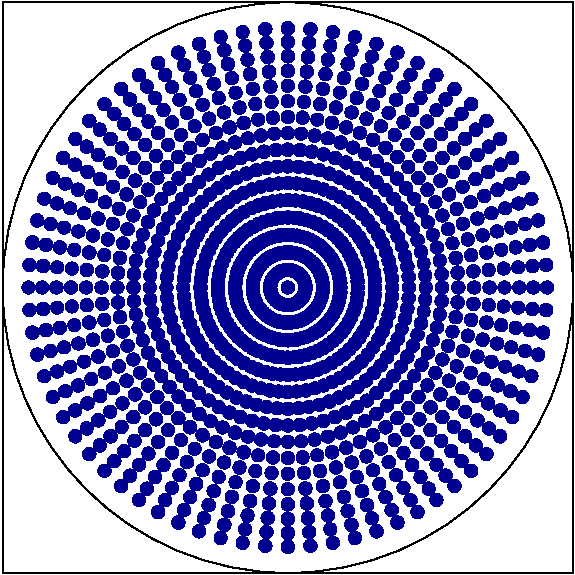
\includegraphics[width=2.5cm]{pic/S2Grid2} \quad
  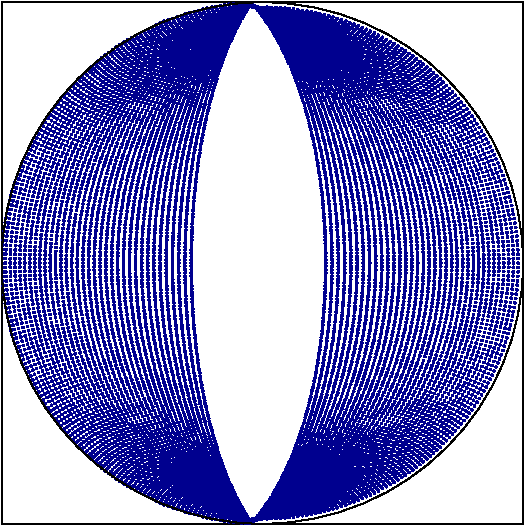
\includegraphics[width=2.5cm]{pic/S2Grid3} \quad
  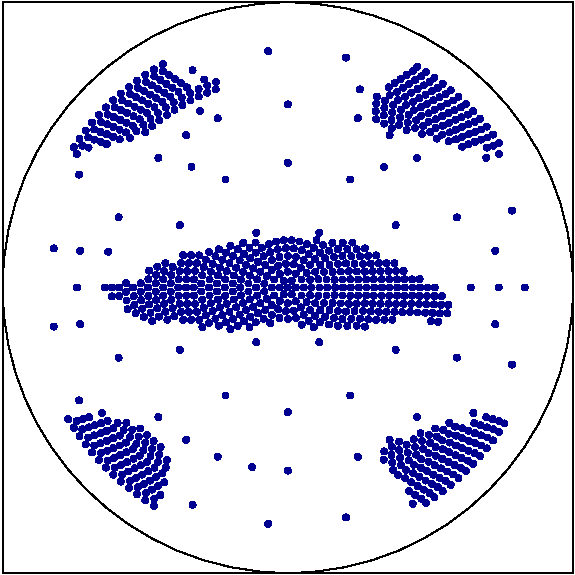
\includegraphics[width=2.5cm]{pic/S2Grid4}
\end{center}

\end{frame}

\subsection*{Exercises}

\begin{frame}

  \begin{Exercise}
    Consider trigonal crystal symmetry.

    \begin{enumerate}[a)]
    \item Find all crystallographic directions symmetrically equivalent to $h
      = (1, 0, \bar 1, 0)$ (Miller indices)!
    \item Find crystallographic directions such that the number of their
      crystallographic equivalent directions on the upper hemisphere (without
      equator) is 1, 3, or 6?
    \item Construct an orientation that rotates the crystallographic
      directions $(0,0,0,1)$ and $(2,\bar 1,\bar 1,0)$ onto the specimen
      directions $(1,0,0)$ and $(0,1,0)$, respectively.
    \item Find all crystallographic equivalent orientations to
      $(45\degree,0\degree,0\degree)$ (Euler angle) and give its Euler angles!
    \item Find all crystallographic equivalent specimen directions to the crystal
      direction $(1,1,\bar 2,1)$ under the orientation
      $(45\degree,0\degree,0\degree)$ (Euler angle)!
    \end{enumerate}

  \end{Exercise}

\end{frame}

%%% Local Variables:
%%% mode: latex
%%% TeX-master: "main"
%%% End:
